% WACV 2027 submission for E-Deflare.
% Content migrated from the authoritative ECCV version.

\documentclass[10pt,twocolumn,letterpaper]{article}

%%%%%%%%% PAPER TYPE
\usepackage[review,algorithms]{wacv}
% \usepackage[review,applications]{wacv}
% \usepackage[review,datasets]{wacv}
% \usepackage{wacv}
% \usepackage[pagenumbers]{wacv}

\usepackage{algorithm}
\usepackage{algpseudocode}
\usepackage{colortbl}
\usepackage{multirow}
\usepackage{wrapfig}
\usepackage{float}
\usepackage{titletoc}
\usepackage{placeins}
\usepackage{soul}

\setlength{\textfloatsep}{8pt plus 2pt minus 2pt}
\setlength{\dbltextfloatsep}{8pt plus 2pt minus 2pt}
\setlength{\floatsep}{6pt plus 2pt minus 2pt}
\setlength{\dblfloatsep}{6pt plus 2pt minus 2pt}

\definecolor{ev_1}{RGB}{247,0,9}
\definecolor{ev_2}{RGB}{214,9,42}
\definecolor{ev_3}{RGB}{196,13,61}
\definecolor{ev_4}{RGB}{156,19,102}
\definecolor{ev_5}{RGB}{102,31,157}
\definecolor{ev_6}{RGB}{101,31,158}
\definecolor{ev_7}{RGB}{66,37,194}
\definecolor{ev_8}{RGB}{49,41,211}
\definecolor{ev_9}{RGB}{28,41,206}

\newcommand{\ours}{\textbf{\textcolor{ev_1}{E}\textcolor{ev_2}{-}\textcolor{ev_3}{D}\textcolor{ev_4}{e}\textcolor{ev_5}{f}\textcolor{ev_6}{l}\textcolor{ev_7}{a}\textcolor{ev_8}{r}\textcolor{ev_9}{e}}}

\definecolor{red}{rgb}{0.8,0,0}
\definecolor{green}{RGB}{0, 133, 21}
\definecolor{grey}{rgb}{0.5,0.5,0.5}

\definecolor{ev_green}{RGB}{0, 180, 139}
\definecolor{ev_red}{RGB}{239, 99, 75}
\definecolor{ev_blue}{RGB}{99, 113, 250}

\newcommand{\mb}[1]{\mathbf{#1}}
\def\tabref#1{Table~\ref{#1}}
\def\figref#1{Figure~\ref{#1}}
\def\secref#1{Section~\ref{#1}}
\def\algref#1{Algorithm~\ref{#1}}
\def\appref#1{Appendix~\ref{#1}}

\newcommand{\Ra}{\textcolor{red}{jp3v}\xspace}
\newcommand{\Rb}{\textcolor{green}{yp7r}\xspace}
\newcommand{\Rc}{\textcolor{blue}{P4hs}\xspace}

\newcommand{\red}[1]{{\color{red}#1}}
\newcommand{\todo}[1]{{\color{red}#1}}
\newcommand{\TODO}[1]{\textbf{\color{red}[TODO: #1]}}


\definecolor{wacvblue}{rgb}{0.21,0.49,0.74}
\usepackage[pagebackref,breaklinks,colorlinks,allcolors=wacvblue]{hyperref}

%%%%%%%%% PAPER ID
\def\wacvPaperID{*****}
\def\confName{WACV}
\def\confYear{2027}

%%%%%%%%% TITLE
\title{Learning to Remove Lens Flare in Event Camera}

%%%%%%%%% AUTHORS
\author{}

\begin{document}

\twocolumn[{
    \renewcommand\twocolumn[1][]{#1}
    \maketitle
    \begin{center}
    \centering
    \captionsetup{type=figure}
    \vspace{-0.7cm}
    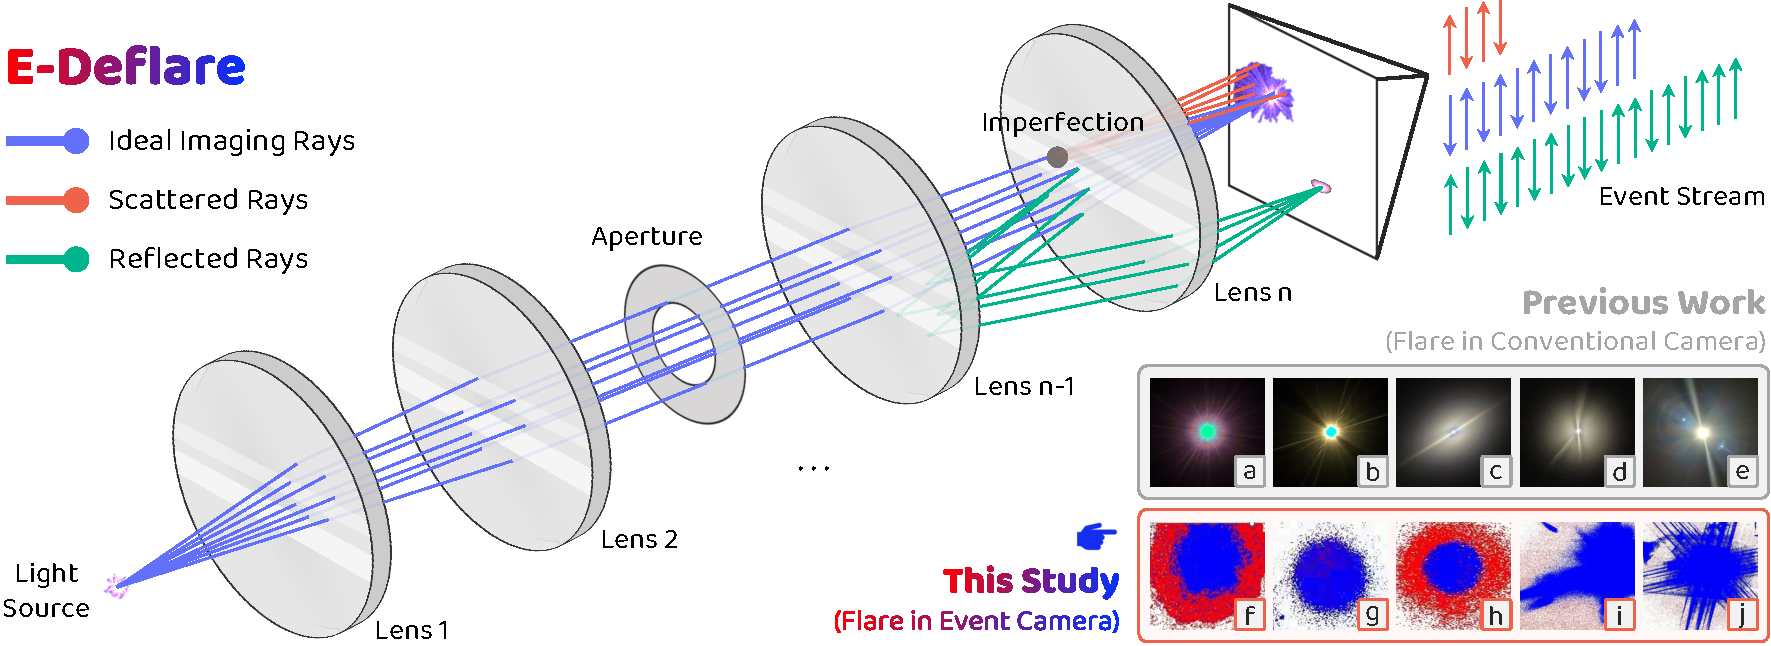
\includegraphics[width=\textwidth]{figures/teaser.pdf}
    \vspace{-0.55cm}
    \caption{\textbf{The physical principle of lens flare and its manifestation in event cameras.} The central diagram deconstructs the universal optical process: ideal \textbf{Imaging Rays} form the scene, while \textbf{Scattered Rays} (from lens imperfections) and \textbf{Internal Reflections} superimpose flare artifacts. While lens flare is a well-studied problem in conventional imaging (\emph{bottom right}, plots $\mathbf{a}$ to $\mathbf{e}$), its complex spatio-temporal manifestation in event data has been largely overlooked (\emph{bottom right}, plots $\mathbf{f}$ to $\mathbf{j}$). Our work is the \textbf{first} to systematically address this challenge. The \textcolor{red}{\textbf{positive}} (brightness increase) and \textcolor{blue}{\textbf{negative}} (brightness decrease) events are colored \textcolor{red}{\textbf{red}} and \textcolor{blue}{\textbf{blue}}, respectively.}
    \label{fig:teaser}
    \vspace{0.2cm}
    \end{center}
}]

\begin{abstract}
Event cameras have the potential to revolutionize vision systems with their high temporal resolution and dynamic range, yet they remain susceptible to lens flare, a fundamental optical artifact that causes severe degradation. In event streams, this optical artifact forms a complex, spatio-temporal distortion that has been largely overlooked. We present \ours, the first systematic framework for removing lens flare from event camera data. We first establish the theoretical foundation by deriving a physics-grounded forward model of the non-linear suppression mechanism. This insight enables the creation of the \textbf{E-Deflare Benchmark}, a comprehensive resource featuring a large-scale simulated training set, \textbf{E-Flare2.7K}, and the first-ever paired real-world test set, \textbf{E-Flare-R}, captured by our novel optical system. Using \textbf{E-DeflareNet}, a standard 3D U-Net restoration network, we show that training on our physically grounded data achieves state-of-the-art performance. Extensive experiments validate our approach and demonstrate clear benefits for downstream tasks. Code and data samples are provided in Supplementary Material.

\end{abstract}

\section{Introduction}
\label{sec:intro}

Lens flare \cite{fowles1989introduction,hullin2011physically,wu2021train}, an optical artifact caused by reflections and scattering within a camera lens, is a well-known source of image degradation in conventional photography \cite{wu2021train,zhou2023improving,dai2022flare7k,dai2024flare7k++,jiang2024mfdnet}. It severely compromises downstream vision tasks and is not fully avoidable by hardware such as lens hoods, which \textbf{cannot block light sources within the field of view}, motivating extensive and ongoing research on lens flare removal in the image domain. 


Event cameras \cite{gallego2020event,li2021recent,posch2014retinomorphic, chaney2023m3ed,perot2020mpx1,kim2021n-imagenet,muglikar2025event}, which asynchronously capture intensity changes at microsecond resolution, are increasingly important for high-speed and high-dynamic-range applications \cite{tulyakov2022time,hagenaars2021self,li2022asynchronous,lin2024e2pnet,vemprala2021representation,wang2023visevent,zheng2023deep,gehrig2024low,han2024event,li2025active,alonso2019ev-segnet,sun2022ess,kong2024openess,kong2025eventfly,kong2025talk2event,lu2025flexevent,sun2024unified,gehrig2024dense,brander2025reading,messikommer2025data,geckeler2025event}. However, their high dynamic range does not extend to seeing through lens flare, whose intensity is superimposed onto the scene irradiance before the sensor, \textbf{rendering the two inseparable} \cite{brandli2014davis,posch2010gen1,son2017gen3,finateu2020gen4}. Flare-like artifacts are present in many widely used event datasets~\cite{gehrig2021dsec,gehrig2021raft,hu2020ddd20,binas2017ddd17,zhu2018multivehicle}, where they degrade data quality and hinder downstream performance~\cite{shi2023identifying,shi2024polarity,hidalgo2020learning,zubic2023from,jing2024hpl-ess,hamaguchi2023hmnet}. These artifacts have been attributed to generic lighting interference~\cite{shi2023identifying}, without recognizing them as lens flare. We argue that lens flare in event cameras is \textbf{a critical yet overlooked problem}. As shown in Fig.~\ref{fig:teaser}, it manifests as a highly structured, spatio-temporal distortion precisely explained by the underlying optics.


This oversight has significant consequences. In event streams, lens flare appears as large-scale, temporally correlated patterns that differ fundamentally from \emph{random noise} or \emph{periodic flickers}. Existing event-based denoising methods \cite{shi2024polarity,shi2023identifying,wang2022linear,guo2022low,duan2021eventzoom}, designed for \emph{uncorrelated} or \emph{uniform noise}, fail to suppress structured artifacts. Moreover, strong flare signals can \textbf{suppress or distort valid background events} \cite{valencia2023optically}. Recovering this corrupted background is akin to event-based see-through \cite{yu2022learning}, yet far more challenging: those methods assume controlled settings in which only the occluder moves, whereas lens flare is an inherently unconstrained corruption present in arbitrary scenes.


A learning-based approach appears most promising, yet it is hindered by a fundamental obstacle: \textbf{the absence of paired training and testing data}~\cite{dai2022flare7k,dai2024flare7k++}. Capturing perfectly aligned event pairs with and without flare requires re-recording the same scene under identical conditions, which is infeasible. This challenge is amplified for event cameras, whose motion encoding makes trajectory alignment nearly impossible. Naively applying an event simulator~\cite{hu2021v2e,lin2022dvs,joubert2021event,zhang2023v2ce,han2024physical} to existing image datasets yields a fully synthetic domain for both input and ground truth, creating a severe sim-to-real gap. Simulation-based approaches in the image domain have addressed this scarcity by collecting flare and background assets \emph{separately}, then compositing them into paired training samples via direct linear superposition~\cite{wu2021train,dai2022flare7k,dai2024flare7k++}, a strategy whose practicality is now well established. The analogous route for event cameras is natural, yet its compositing step is categorically different. Event cameras encode irradiance in the logarithmic domain, merging background and flare event streams is \textbf{not a simple union but a non-linear suppression process} that has never been formally analyzed or characterized.



We introduce \emph{\ours}, a framework that resolves this challenge by grounding the data generation pipeline in physical analysis. We derive a physical forward model revealing the non-linear compositing mechanism at the core of this problem, which directly guides our primary contributions: a physics-driven simulator that generates the large-scale \textbf{E-Flare2.7K} training set, and a novel, physically-principled acquisition system that captures \textbf{E-Flare-R}, the first-ever paired real-world test set. This benchmark enables training \textbf{E-DeflareNet}, a standard 3D U-Net restoration network, to restore clean event streams with high fidelity.


Our main contributions can be summarized as follows:
\begin{itemize}
    \item To our knowledge, we are the first to provide a rigorous physical analysis of lens flare in event data, culminating in a \textbf{forward model} that formalizes the non-linear suppression mechanism underlying event stream corruption. This builds a theoretical foundation for de-flaring tasks in event-based vision.

    \item Guided by our physical model, we introduce the first \textbf{simulation pipeline} that explicitly models non-linear flare corruption in event streams, enabling large-scale, physically-grounded paired training data for the first time.

    \item We design and contribute the \textbf{E-Deflare Benchmark}, the first comprehensive resource for the event camera de-flaring task, comprising a large-scale simulated dataset (\emph{E-Flare2.7K}), a curated set of real-world examples (\emph{DSEC-Flare}), and critically, the first-ever paired \textbf{real-world test set} (\emph{E-Flare-R}) for comprehensive evaluations and assessments.

    \item We use a standard 3D U-Net, \textbf{E-DeflareNet}, to validate the proposed physical formulation and paired data, showing that training on our data yields strong de-flaring performance and improves downstream event camera imaging.
\end{itemize}



















% Lens flare \cite{fowles1989introduction,hullin2011physically,wu2021train}, an optical artifact from internal scattering and reflections within a camera's lens, is a well-known source of degradation in conventional photography~\cite{wu2021train,zhou2023improving,dai2022flare7k,dai2024flare7k++,jiang2024mfdnet}. It severely compromises downstream computer vision tasks, motivating substantial research on flare removal in the image domain. Event cameras~\cite{gallego2020event, li2021recent, posch2014retinomorphic}, which asynchronously record light changes at the microsecond level, are increasingly critical in challenging vision tasks~\cite{tulyakov2022time,hagenaars2021self, li2022asynchronous, lin2024e2pnet, vemprala2021representation, wang2023visevent, zheng2023deep,gehrig2024low,han2024event,li2025active}. While their unique sensing paradigm offers advantages like high dynamic range, they are not immune to this fundamental optical limitation. Indeed, flare-like artifacts are visibly present in many prominent event camera datasets~\cite{gehrig2021dsec,gehrig2021raft,hu2020ddd20,binas2017ddd17,zhu2018multivehicle}, where they degrade data quality and affect downstream tasks~\cite{shi2023identifying,shi2024polarity,hidalgo2020learning}. However, these artifacts have generally been attributed to generic light source interference~\cite{shi2023identifying}, without a systematic analysis that identifies them as the distinct optical phenomenon of physical lens flare. We argue that lens flare in event cameras is a critical and overlooked problem. As illustrated in Fig.~\ref{fig:teaser}, it manifests as a highly complex spatio-temporal phenomenon, whose intricate patterns can be precisely explained by the underlying physics of lens flare.

% This oversight has significant consequences. In event streams, lens flare manifests as large-scale, complex, and \textbf{spatio-temporally correlated} patterns. Existing event-based denoising methods~\cite{shi2024polarity, shi2023identifying, wang2022linear,guo2022low,duan2021eventzoom}, designed for random, uncorrelated noise or uniform flicker, are fundamentally ill-equipped to handle such structured artifacts. The contamination is not limited to adding spurious activity; as our theoretical analysis will explain, the strong flare signal can also suppress and distort legitimate event data from the background~\cite{muglikar2025event,valencia2023optically}, making the de-flaring task even more difficult.

% To tackle such a complex artifact, a learning-based approach is the most promising path. However, this path is blocked by a fundamental obstacle: the absence of suitable training and testing data~\cite{dai2022flare7k,dai2024flare7k++}. Generating large-scale, perfectly-aligned paired data would require capturing a dynamic scene twice with pixel-perfect alignment—once with flare and once without. This is an extremely difficult task, as one cannot simply disable the optical effect without altering the scene's illumination, nor can one perfectly replicate the precise trajectory of any moving objects. This data acquisition challenge is even more severe for event cameras, which inherently capture dynamic information~\cite{gallego2020event}, making the alignment of trajectories exceptionally difficult. Furthermore, a naive workaround, such as applying an event simulator~\cite{hu2021v2e,lin2022dvs,joubert2021event,zhang2023v2ce,han2024physical} to existing paired frame datasets, is also untenable, as it would create a fully simulated dataset for both input and ground truth, introducing a significant sim-to-real gap.

% To break this data deadlock, this paper presents \textbf{E-Deflare}, a systematic framework built upon a rigorous, physics-driven methodology. Our approach is founded on a deep analysis of the underlying optical principles, which enables a complete solution from theory to practice. We first establish a theoretical foundation for the problem, then leverage it to engineer a data-centric solution that makes learning-based de-flaring possible. We demonstrate the success of this framework by training a 3D U-Net-based architecture~\cite{10.7554/eLife.57613,cciccek20163d,lee2017superhuman} to effectively restore clean event streams.

% Our main contributions are as follows:
% \begin{itemize}
%     \item \textbf{Theoretical Foundation.} We are the first to systematically identify lens flare in event cameras and derive a theoretical \textbf{forward model} that explains how it contaminates event streams via a non-linear suppression mechanism. This provides the physical basis for designing effective de-flaring strategies.
    
%     \item \textbf{Simulation for Training.} Based on our model, we build the first physics-driven \textbf{simulation pipeline} to generate a large-scale, paired dataset. This overcomes the primary bottleneck for training deep de-flaring networks.
    
%     \item \textbf{Real-World Validation and Benchmark.} We propose a novel method to acquire a paired \textbf{real-world test set}, enabling robust validation of sim-to-real generalization. We will release our synthetic and real datasets as the first public \textbf{benchmark} to foster future research in this area.
% \end{itemize}

\section{Related Work}
\label{sec:related_work}

\noindent\textbf{Lens Flare Removal.}
Lens flare is a long-standing problem in image restoration, caused by reflections and scattering within camera lenses \cite{fowles1989introduction,hullin2011physically,wu2021train}. Early heuristic methods \cite{asha2019auto,vitoria2019automatic} have been surpassed by learning-based approaches \cite{dai2023nighttime,dai2022flare7k,wu2021train,dai2024flare7k++,zhou2023improving,jiang2024mfdnet}, which achieve superior performance but face the same challenge: \textit{the lack of paired real-world data} \cite{dai2022flare7k,wu2021train}. This constraint has led to two main directions: unpaired learning with generative models \cite{qiao2021light}, often sacrificing detail, and synthetic training using simulated flare layers \cite{wu2021train,dai2022flare7k,dai2024flare7k++,zhou2023improving}. These simulation-based pipelines are practical when paired data are scarce, yet they share a common assumption: that training pairs can be synthesized by linearly superimposing flare onto clean images. This additive assumption does not hold for event cameras, which inherently encode intensity in a non-linear and discrete manner; to our knowledge, we are the first to characterize this non-linear effect and account for it in a simulation pipeline. Yet, all existing methods target static images; they neither address the asynchronous, high-temporal-resolution nature of event data nor the dynamic behavior of flare in this setting.


\noindent\textbf{Event Artifact Removal.}
Event stream restoration has targeted a variety of artifacts. Previous works remove sensor noise such as background activity using hand-crafted filters \cite{shi2024polarity,wu2020probabilistic,guo2022low,feng2020event,wang2019ev,wang2020joint} or learning-based techniques \cite{duan2021eventzoom,rios2023within,baldwin2020event,duan2021guided,zhang2023neuromorphic}. These methods handle random or uncorrelated noise, fundamentally different from the structured patterns caused by lens flare. Others focus on interference from light sources, \eg, flicker removal \cite{wang2022linear,im2023live}, but flare can arise even under stable illumination, making such filters inadequate. A few works mention ``stray light'' artifacts \cite{shi2023identifying,shi2024polarity}, closely related to flare, yet treat them as generic light interference without a physical model. Without a physical model, such filters risk suppressing valid events. In contrast, we explicitly model flare as a distinct optical phenomenon and address it with a physics-guided approach.


\noindent\textbf{Event Camera Simulation.}
The scarcity of ground-truth event data has motivated the development of event simulators \cite{bhattacharya2025monocular,messikommer2025data,pellerito2024deep,muglikar2023event}, generally classified into video-driven and learning-based approaches. However, neither can produce paired flare data. The video-driven simulators \cite{rebecq2018esim,hu2021v2e,gehrig2020video,joubert2021event,lin2022dvs,han2024physical} rely on input videos, but paired video flare datasets do not exist, and these methods already suffer from notable sim-to-real gaps \cite{stoffregen2020reducing}, which would worsen when converting synthetic flare videos to synthetic events. Learning-based simulators \cite{zhang2023v2ce,gehrig2020video,pantho2022event,baek2020real,rizzo2022event,zhu2021eventgan,gu2021learn} depend on large and diverse training data that are currently unavailable for flare modeling. Consequently, to the best of our knowledge, \emph{no existing simulator explicitly models lens flare in event cameras;} we introduce the \textbf{first} physics-based simulator derived from an explicit analytical flare formation model for events.











\section{Methodology}
\label{sec:methodology}
This section introduces \emph{\ours}, a physics-guided approach for removing lens flare in event cameras. We derive a \textbf{forward model} of flare formation, whose exact inversion is intractable (Sec.~\ref{ssec:forward_model}), motivating a learning-based solution. Building on this, we develop a two-stage strategy: a \textbf{physics-driven simulator} for large-scale paired training data (Sec.~\ref{ssec:simulator}) and a \textbf{real-world acquisition system} for robust validation (Sec.~\ref{ssec:real_data_acquisition}). We then define the learning objective and restoration network. The overview framework is illustrated in Fig.~\ref{fig:methodology-flowchart}.


\begin{figure*}[!t]
    \centering
    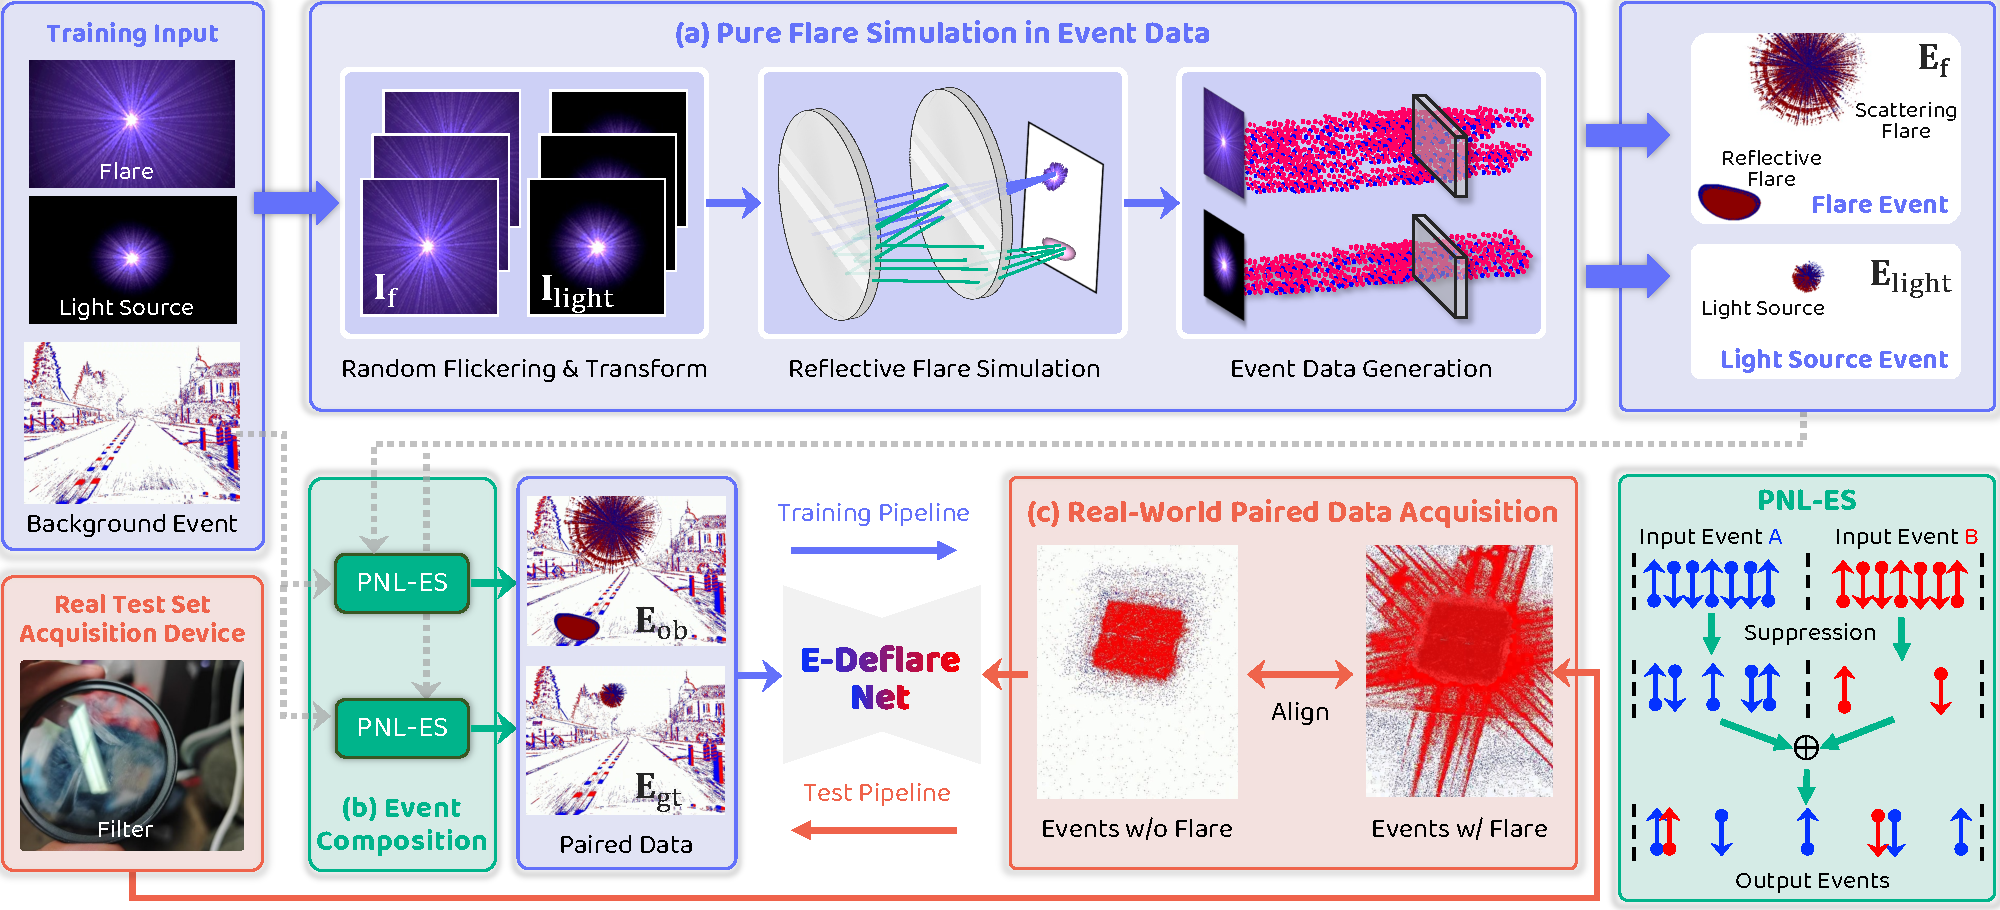
\includegraphics[width=\textwidth]{figures/pipeline.pdf}
    \vspace{-0.5cm}
    \caption{\textbf{Data Generation, Training \& Validation.} 
    In the \emph{\ours}~framework, we introduce two parallel pipelines to address data scarcity. 
    The training pipeline synthesizes paired data by first generating dynamic flare events from static images (\eg, Flare7K++) and then fusing them with real background events (\eg, DSEC) via our physics-guided PNL-ES operator. 
    The testing pipeline captures paired real-world data using a controllable optical setup. A removable filter allows us to record the same dynamic scene \emph{w/} and \emph{w/o} flare, which forms our validation set after post-processing.
    }
    \vspace{-0.2cm}
    \label{fig:methodology-flowchart}
\end{figure*}



\subsection{Physical Modeling of Flare in Events}
\label{ssec:forward_model}

To model lens flare in event streams, we establish a physical model of the \emph{scene} and \emph{imaging process}, decomposing the total irradiance into background $\mathbf{I}_{\mathrm{bg}}$ and a primary light source $\mathbf{I}_{\mathrm{light}}$. Under an \textbf{ideal lens} $\mathcal{L}_{\mathrm{ideal}}$, both components are perfectly imaged, producing the clean, flare-free ground-truth irradiance:
\begin{equation}
    \mathbf{I}_{\mathrm{gt}}(x, y, t) = \mathbf{I}_{\mathrm{bg}}(x, y, t) + \mathbf{I}_{\mathrm{light}}(x, y, t)~.
\end{equation}
In contrast, a \textbf{real lens} $\mathcal{L}_{\mathrm{real}}$ introduces reflections and scattering that corrupt this formation. While the background remains largely unaffected, the bright light source produces a spatially expansive, structured flare component $\mathbf{I}_{\textcolor{ev_red}{\mathrm{\mathbf{f}}}}$ that subsumes both the distorted direct illumination and the additional scattered energy, thereby replacing $\mathbf{I}_{\mathrm{light}}$ in the observed irradiance. The observed irradiance $\mathbf{I}_{\mathrm{ob}}$ can thus be approximated by a linear superposition in the intensity domain~\cite{dai2022flare7k,wu2021train,dai2024flare7k++}. This process is formulated as follows:
\begin{equation}
    \mathbf{I}_{\mathrm{ob}}(x, y, t) \approx \mathbf{I}_{\mathrm{bg}}(x, y, t) + \mathbf{I}_{\textcolor{ev_red}{\mathrm{\mathbf{f}}}}(x, y, t)~.
\label{eq:image_superposition_final}
\end{equation}
This intensity-domain corruption occurs \emph{before} the sensor and forms the foundation of our event-level analysis. For brevity, we omit coordinates $(x, y)$ where context is clear.

An event camera sensor $\mathcal{S}_{\mathrm{evt}}(\cdot)$ operates on this corrupted irradiance $\mathbf{I}_{\mathrm{ob}}$. Unlike conventional cameras that capture frames at fixed intervals, $\mathcal{S}_{\mathrm{evt}}$ is a stateful process: each pixel independently monitors its log-intensity $L(t) = \log(\mathbf{I}_{\mathrm{ob}}(t))$ and asynchronously triggers an event when the accumulated change exceeds a contrast threshold $c$. Mathematically, an event is fired at time $t_i$ when:
\begin{equation}
    |L(t_i) - L(t_{\mathrm{last}})| \ge c~,
    \label{eq:event_threshold_condition}
\end{equation}
where $t_{\mathrm{last}}$ denotes the timestamp of the preceding event at that pixel. The polarity $p_i = \mathrm{sign}(L(t_i) - L(t_{\mathrm{last}})) \in \{+1, -1\}$ encodes the direction of the intensity change. The resulting event stream $\mathbf{E}(t)$ can be represented as:
\begin{equation}
    \mathbf{E}(t) = \mathcal{S}_{\mathrm{evt}}(\mathbf{I}_{\mathrm{ob}}(t)) = \sum\nolimits_{i} p_i \delta(t - t_i)~,
    \label{eq:event_stream_definition}
\end{equation}
where $\delta(\cdot)$ is the Dirac delta function. This yields an integral relationship between log-intensity and $\mathbf{E}(t)$:
\begin{equation}
    L(t) = c \int_{0}^{t} \mathbf{E}(\tau) \, d\tau + L(0) + \varepsilon(t)~,
    \label{eq:sensor_model_integral_redef}
\end{equation}
where $L(0)$ is the initial log-intensity and $\varepsilon(t)$ represents the \emph{total intensity residual}. This term aggregates all signal components not encoded in the event stream. It mainly comprises two parts: \textbf{(1)} the \textbf{sub-threshold quantization error}, which is bounded by the threshold $c$, and \textbf{(2)} \textbf{sensor noise} (\eg, shot noise, threshold variance), which is stochastic and may accumulate over time. While modern sensors strive to minimize noise, $\varepsilon(t)$ remains an intrinsic and unavoidable part of the underlying physical process.

\textbf{Dual Mathematical Representation.} To establish the physical interaction mechanism between background and flare events, we first recognize that the event stream $\mathbf{E}(t)$, though discrete, admits a continuous interpretation through its temporal derivative relationship. Differentiating Eq.~\ref{eq:sensor_model_integral_redef}, the rate of change of log-intensity can be expressed as:
\begin{equation}
    \frac{dL(t)}{dt} = c \cdot \mathbf{E}(t) + \xi(t)~,
    \label{eq:continuous_link}
\end{equation}
where $\xi(t) \triangleq d\varepsilon(t)/dt$ is the \emph{residual rate}. Eq.~\ref{eq:continuous_link} bridges the discrete and continuous domains.


\textbf{Log-Derivative Mixing.} The linear superposition of irradiance (Eq.~\ref{eq:image_superposition_final}) becomes highly non-linear when mapped to the logarithmic domain. Differentiating $L_{\mathrm{ob}}(t) = \log(\mathbf{I}_{\mathrm{bg}}(t) + \mathbf{I}_{\textcolor{ev_red}{\mathrm{\mathbf{f}}}}(t))$ via the chain rule gives:
\begin{equation}
    \frac{dL_{\mathrm{ob}}(t)}{dt} = w_{\mathrm{bg}}(t) \frac{dL_{\mathrm{bg}}(t)}{dt} + w_{\textcolor{ev_red}{\mathrm{\mathbf{f}}}}(t) \frac{dL_{\textcolor{ev_red}{\mathrm{\mathbf{f}}}}(t)}{dt}~,
    \label{eq:log_derivative_mixing}
\end{equation}
where $L_{\mathrm{bg}}(t) \triangleq \log \mathbf{I}_{\mathrm{bg}}(t)$ and $L_{\textcolor{ev_red}{\mathrm{\mathbf{f}}}}(t) \triangleq \log \mathbf{I}_{\textcolor{ev_red}{\mathrm{\mathbf{f}}}}(t)$, and the coefficients are defined as:
\begin{equation}
    w_{\mathrm{bg}}(t) = \frac{\mathbf{I}_{\mathrm{bg}}(t)}{\mathbf{I}_{\mathrm{bg}}(t) + \mathbf{I}_{\textcolor{ev_red}{\mathrm{\mathbf{f}}}}(t)}~,~~ w_{\textcolor{ev_red}{\mathrm{\mathbf{f}}}}(t) = 1-w_{\mathrm{bg}}(t)~.
    \label{eq:weights_definition}
\end{equation}
This reveals that although intensities superpose linearly, their logarithmic derivatives mix through a weighted sum: the physical origin of the \textbf{non-linear suppression effect}.


\textbf{Complete Forward Model.} Substituting the dual representation (\ie, Eq.~\ref{eq:continuous_link}) into Eq.~\ref{eq:log_derivative_mixing}, we obtain:
\begin{equation}
    \begin{aligned}
    \frac{dL_{\mathrm{ob}}(t)}{dt} ={}&
    w_{\mathrm{bg}}(t) \left[ c \mathbf{E}_{\mathrm{bg}}(t) + \xi_{\mathrm{bg}}(t) \right] \\
    &+ w_{\textcolor{ev_red}{\mathrm{\mathbf{f}}}}(t)
    \left[ c \mathbf{E}_{\textcolor{ev_red}{\mathrm{\mathbf{f}}}}(t)
    + \xi_{\textcolor{ev_red}{\mathrm{\mathbf{f}}}}(t) \right]~,
    \end{aligned}
    \label{eq:full_mixing_derivative}
\end{equation}
where $\xi_{\mathrm{bg}}(t)$ and $\xi_{\textcolor{ev_red}{\mathrm{\mathbf{f}}}}(t)$ denote the respective residual rates. Integrating Eq.~\ref{eq:full_mixing_derivative} over time and substituting back into the sensor model (Eq.~\ref{eq:sensor_model_integral_redef}) yields the complete forward model:
\begin{equation}
    \mathbf{E}_{\mathrm{ob}}(t) = \mathcal{S}_{\mathrm{evt}}\left( \exp\left( \int_{0}^{t} \Phi(\tau) \, d\tau + L_{\mathrm{ob}}(0) \right) \right)~,
    \label{eq:full_forward_model}
\end{equation}
where the integrand $\Phi(\tau)$ represents:
\begin{equation}
    \begin{aligned}
    \Phi(\tau) ={}&
    w_{\mathrm{bg}}(\tau)\, c \mathbf{E}_{\mathrm{bg}}(\tau)
    + w_{\textcolor{ev_red}{\mathrm{\mathbf{f}}}}(\tau)\, c \mathbf{E}_{\textcolor{ev_red}{\mathrm{\mathbf{f}}}}(\tau) \\
    &+ w_{\mathrm{bg}}(\tau)\,\xi_{\mathrm{bg}}(\tau)
    + w_{\textcolor{ev_red}{\mathrm{\mathbf{f}}}}(\tau)\,\xi_{\textcolor{ev_red}{\mathrm{\mathbf{f}}}}(\tau)~.
    \end{aligned}
    \label{eq:integrand_phi}
\end{equation}
The first line contains the weighted impulse terms, and the second line contains the mixed residuals $\xi_{\mathrm{mix}}$. This formulation is physically complete: the outer operator $\mathcal{S}_{\mathrm{evt}}$ ensures the output is a discrete event stream (Eq.~\ref{eq:event_stream_definition}), while the integral captures the accumulated log-intensity change, explaining why flare-dominated regions exhibit slower accumulation, and thus suppressed background events.


\textbf{Practical Considerations.} If continuous irradiance profiles $\mathbf{I}_{\mathrm{bg}}(t)$ and $\mathbf{I}_{\textcolor{ev_red}{\mathrm{\mathbf{f}}}}(t)$ were known, one could compute $w(t)$ and $\xi_{\mathrm{mix}}$ and evaluate $\mathcal{S}_{\mathrm{evt}}$ exactly. In practice, however, complete and accurate irradiance information is unavailable, so $\mathbf{I}(t)$, the weights, and the residual terms cannot be recovered. Exact integration is therefore intractable, motivating the discrete approximation in Sec.~\ref{ssec:simulator}.



\subsection{Physics-Driven Simulator for Paired Data}
\label{ssec:simulator}


As illustrated in Fig.~\ref{fig:methodology-flowchart}, the pipeline operates in two stages: \textbf{Stage 1} generates pure flare events by extending image-based methods~\cite{dai2024flare7k++} to the event domain, while \textbf{Stage 2 implements the physics-driven event composition mechanism}, the core contribution of this work.


$\bullet$~\textbf{Stage 1: Pure Flare Simulation in Events.}
The first stage synthesizes pure event streams for the light source under a non-ideal lens ($\mathbf{E}_{\textcolor{ev_red}{\mathrm{\mathbf{f}}}}$) and an ideal lens ($\mathbf{E}_{\mathrm{light}}$). Real paired dynamic captures would be ideal but are scarce; even image-domain paired flare videos are rare. We therefore use Flare7K++ \cite{dai2024flare7k++}, the only training-scale paired source, and animate its static assets.

To address this, we decompose the flare into two components. For the \textbf{scattering flare}, whose pattern varies smoothly with the light source's position, we generate dynamic videos by applying complex temporal effects to the static Flare7K++ assets. These include random spatial transformations and intensity flickering. For the \textbf{reflective flare}, whose intricate patterns change drastically and cannot be realistically interpolated from static images, we use a dedicated \textbf{Reflective Flare Simulation} module to synthesize its dynamic intensity video. The final video sums both components. These are processed by a standard event simulator~\cite{lin2022dvs} to produce $\mathbf{E}_{\textcolor{ev_red}{\mathrm{\mathbf{f}}}}$ and $\mathbf{E}_{\mathrm{light}}$.


$\bullet$~\textbf{Stage 2: Physics-Driven Event Composition.}
As established in Sec.~\ref{ssec:forward_model}, exactly evaluating the forward model requires continuous irradiance $\mathbf{I}(t)$, which is unavailable during synthesis. A naive heuristic is to directly merge the two streams ($\mathbf{E}_{\mathrm{ob}} \approx \mathbf{E}_{\mathrm{bg}} \cup \mathbf{E}_{\textcolor{ev_red}{\mathrm{\mathbf{f}}}}$), which implicitly assumes $w_{\mathrm{bg}} = w_{\textcolor{ev_red}{\mathrm{\mathbf{f}}}} = 1$ and ignores the normalized weighting entirely. This is physically incorrect: in the extreme case where flare irradiance dominates ($\mathbf{I}_{\textcolor{ev_red}{\mathrm{\mathbf{f}}}} \gg \mathbf{I}_{\mathrm{bg}}$), the physical weight $w_{\mathrm{bg}} \to 0$ and background events should be almost entirely suppressed. Direct addition erroneously preserves all of them, producing training data that fundamentally misrepresents the sensor response.

To implement the physical weighting under this constraint, we introduce the \emph{Probabilistic Non-Linear Event Suppression} (\textbf{PNL-ES}) operator $\oplus$. PNL-ES independently retains each background event with probability $w_{\mathrm{bg}}(t)$ and each flare event with probability $w_{\textcolor{ev_red}{\mathrm{\mathbf{f}}}}(t)$, then combines the survivors into a single stream; this is fundamentally different from direct union, which implicitly sets both probabilities to one and discards the weighting. The physical justification follows from Eq.~\ref{eq:full_mixing_derivative}: each background impulse advances $L_{\mathrm{ob}}$ by only $w_{\mathrm{bg}}(t)\cdot c$ rather than the full threshold $c$, so the expected fraction of background events surviving to trigger an observed event is exactly $w_{\mathrm{bg}}(t)$. As a concrete example, when $\mathbf{I}_{\textcolor{ev_red}{\mathrm{\mathbf{f}}}} \gg \mathbf{I}_{\mathrm{bg}}$ (a common scenario near bright light sources), $w_{\mathrm{bg}} \to 0$ and background events should be nearly eliminated; direct union would erroneously preserve all of them. Since continuous $\mathbf{I}(t)$ is unavailable, we estimate the weights from intensity proxies; because PNL-ES is probabilistic, inexact estimates do not yield a single incorrect simulation but instead produce varied training samples spanning a realistic distribution of suppression states, providing principled physics-guided augmentation rather than a deterministic reconstruction.

Using this operator, we construct both the flare-corrupted input and its corresponding clean ground truth, that is:
\begin{equation}
    \mathbf{E}_{\mathrm{ob}} = \mathbf{E}_{\mathrm{bg}} \oplus \mathbf{E}_{\textcolor{ev_red}{\mathrm{\mathbf{f}}}} , \quad
\mathbf{E}_{\mathrm{gt}} = \mathbf{E}_{\mathrm{bg}} \oplus \mathbf{E}_{\mathrm{light}}~.
\end{equation}
The required data assets are assembled accordingly. Real-world background events $\mathbf{E}_{\mathrm{bg}}$ with diverse real-world motion are sampled from DSEC~\cite{gehrig2021dsec}, while intensity profiles for retention probability are obtained from Stage 1's synthetic outputs ($\mathbf{I}_{\textcolor{ev_red}{\mathrm{\mathbf{f}}}}$ and $\mathbf{I}_{\mathrm{light}}$) and estimated from the available event data ($\mathbf{I}_{\mathrm{bg}}$), all of which are sufficient for the probabilistic PNL-ES formulation.


This pipeline yields a large-scale, physically grounded training dataset. By anchoring synthesis to real background events (which dominate event density), we mitigate the sim-to-real gap of fully synthetic systems. As validated below, this facilitates generalization to \emph{real-world} data.



\subsection{Real-World Paired Data Acquisition}
\label{ssec:real_data_acquisition}

Validation faces the practical impossibility of capturing \emph{perfectly aligned} scene pairs with and without flare. Inspired by image-based strategies~\cite{dai2022flare7k, dai2024flare7k++}, we adapt this general capture strategy to event cameras.

\textbf{Capture Setup.} We mount a removable optical filter (\eg, six-line star filters) in front of the lens (Fig.~\ref{fig:methodology-flowchart}). The protocol involves two consecutive recordings of the same scene: one with the filter in place to capture the flare-corrupted stream $\mathbf{E}_{\mathrm{ob}}$, and another immediately after its removal to acquire the near-clean reference $\tilde{\mathbf{E}}_{\mathrm{gt}}$. Multiple filter types introduce diversity in flare patterns.

\textbf{Event-Specific Alignment Strategy.} Unlike frame-based cameras, event cameras possess microsecond-level temporal sensitivity, making precise alignment difficult if either the camera or the scene moves; this is why no such paired dataset currently exists. To address this, we fix the camera and illuminate with high-frequency flickering light sources (\eg, LED arrays). Spatial alignment follows automatically; temporal alignment is achieved by synchronizing streams to the flickering pattern. This yields a small-scale but high-fidelity real-world validation set.

\begin{figure}[!t]
    \centering
    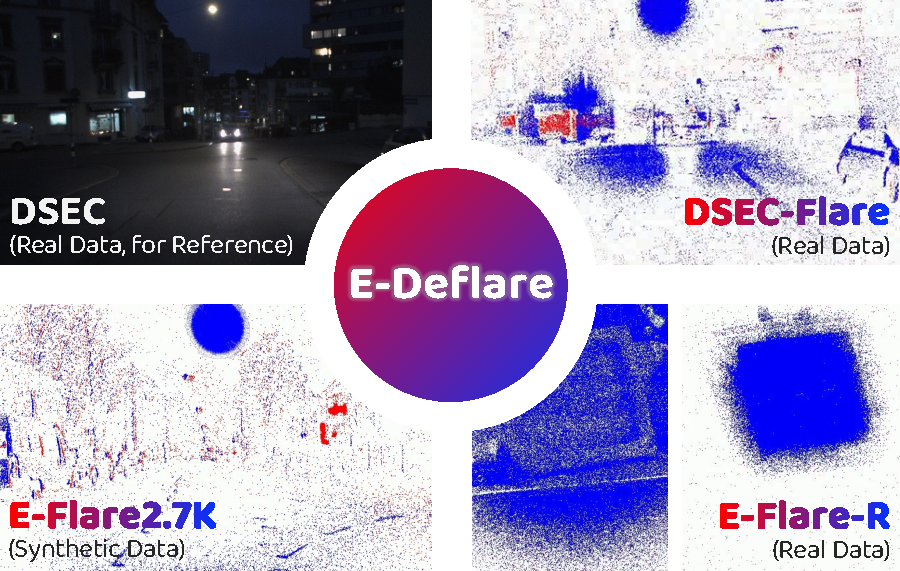
\includegraphics[width=\columnwidth]{figures/2x2.pdf}
    \vspace{-0.65cm}
    \caption{Data samples from our benchmark, shown alongside a reference RGB frame (top left). The benchmark includes: a real-world flare example from \textbf{DSEC-Flare} (top right); a synthetic sample from \textbf{E-Flare2.7K} (bottom left); and a paired real-world sample from our test set \textbf{E-Flare-R} (bottom right).}
    \label{fig:2x2}
\end{figure}
\textbf{Post-Processing.} The captured stream $\tilde{\mathbf{E}}_{\mathrm{gt}}$ undergoes residual artifact suppression (facilitated by the known light source geometry) and metric-guided spatio-temporal refinement to yield the final ground truth $\mathbf{E}_{\mathrm{gt}}$. While this protocol is designed for controlled validation and does not cover scenarios involving camera or scene motion, we complement it with DSEC-Flare, a large-scale collection of unpaired real-world flare examples mined from public datasets. Though lacking ground-truth alignment, DSEC-Flare provides diverse and challenging flare patterns that allow qualitative assessment of generalization beyond controlled settings, thus serving as a complementary benchmark to our paired test set.


We then train E-DeflareNet to validate our data pipeline and theoretical analysis. Event streams are converted to voxel grids $\mathcal{V}(\cdot)$~\cite{duan2021eventzoom}. Using a standard 3D U-Net~\cite{cciccek20163d} with residual prediction, we optimize:
\begin{equation}
\theta^* = \underset{\theta}{\arg\min} \left\| \mathcal{V}(\mathbf{E}_{\mathrm{ob}}) + f_{\theta}(\mathcal{V}(\mathbf{E}_{\mathrm{ob}})) - \mathcal{V}(\mathbf{E}_{\mathrm{gt}}) \right\|_2^2.
\end{equation}
The restored voxel grid is $\hat{\mathcal{V}}_{\mathrm{gt}} = \mathcal{V}(\mathbf{E}_{\mathrm{ob}}) + f_{\theta}(\mathcal{V}(\mathbf{E}_{\mathrm{ob}}))$. 
% Details are in the \textbf{Appendix}.


\subsection{Datasets \& Benchmark}
The \emph{\ours}~benchmark comprises three complementary datasets, each serving a distinct role:
\begin{itemize}
    \item \textbf{\underline{E-Flare2.7K}:} A large-scale \emph{simulated} dataset for training and quantitative testing, with $2.7$K samples ($2{,}545$ training, $175$ testing). Light-source positions and flare patterns are randomized; see the \textbf{Appendix} for examples.

    \item \textbf{\underline{E-Flare-R}:} A paired \emph{real-world} test set for high-fidelity validation under controlled acquisition, providing $150$ samples with optical artifacts such as surface glare and internal reflections~\cite{shi2023identifying}.

    \item \textbf{\underline{DSEC-Flare}:} Curated sequences from the public DSEC dataset~\cite{gehrig2021dsec} exhibiting natural flare corruption in driving scenarios, used for qualitative real-world evaluation where paired ground truth is not needed.
\end{itemize}

\iffalse
\begin{table}[!t]
    \centering
    \small
    \caption{Overview of the proposed datasets in \emph{\ours}~benchmark.}
    \vspace{0.1cm}
    \label{tab:dataset_overview}
    \begin{tabular}{lccc}
    \toprule
    \textbf{Dataset} & \textbf{Type} & \textbf{Paired} & \textbf{Bkg.} \\
    \midrule
    E-Flare2.7K & Synth. & \checkmark & \checkmark \\
    E-Flare-R   & Real   & \checkmark & --         \\
    DSEC-Flare  & Real   & --         & \checkmark \\
    \bottomrule
    \end{tabular}
    \vspace{-0.2cm}
\end{table}
\fi
Together, these datasets cover large-scale learning, paired real-world evaluation, and qualitative evidence in natural driving scenes, which cannot be obtained from a single acquisition source. Some representative data samples are in \cref{fig:2x2}. Further details are provided in the \textbf{Appendix}.

\section{Experiments}
\label{sec:experiments}
This section presents quantitative \& qualitative experiments on event de-flaring.

\subsection{Experimental Settings}

Our proposed model is trained exclusively on \emph{E-Flare2.7K-train}, and tested on \emph{E-Flare2.7K-test}, \emph{E-Flare-R}, and \emph{DSEC-Flare} datasets, respectively.


\noindent\textbf{Baselines.}
Image-based flare removal methods~\cite{wu2021train,dai2022flare7k,dai2024flare7k++,zhou2023improving} are not directly applicable to event streams, as they operate on dense pixel frames; adapting them would require a non-trivial domain translation that is itself an open problem. We instead compare against five representative baselines: (1) the unprocessed \emph{RAW Input}; (2) \emph{Voxel Transform}, a round-trip codec baseline that encodes events into voxel grids and decodes them back without any learned processing, isolating the effect of the representation itself; (3) \emph{EFR}~\cite{wang2022linear}, a classical flicker-removal filter; and (4–5) two recent denoising variants from~\cite{shi2024polarity}: \emph{PFD-A} (general noise suppression) and \emph{PFD-B} (light-interference mitigation). Due to space limitations, more details are provided in the \textbf{Appendix}.


\noindent\textbf{Evaluation Protocol.} 
As no established metrics exist for this task, we adapt measures from related event-based studies.  
For \textbf{event-level} fidelity, inspired by PECS~\cite{han2024physical}, we design two metrics: the \emph{Chamfer Distance} ($\downarrow$), the average nearest-neighbor distance to ground-truth events; and the \emph{Gaussian Distance} ($\downarrow$), applying Gaussian weighting to suppress outliers. For \textbf{voxel-level} structural quality, we adopt the standard evaluation suite from V2CE~\cite{zhang2023v2ce}, including \emph{Mean Squared Error} (MSE, $\downarrow$), \emph{Pooled MSE} (PMSE, $\downarrow$), and \emph{Binarized-Grid F1} scores (R-F1, T-F1, TP-F1, all $\uparrow$) to jointly and comprehensively capture reconstruction accuracy and overall precision-recall balance.


\noindent\textbf{Implementation Details.} 
Our model is trained on \textbf{E-Flare2.7K} for $40$k iterations on a single NVIDIA RTX $3090$ GPU. The network employs a standard residual 3D U-Net, demonstrating that our physically grounded data alone suffice for effective learning. Due to space limitations, more implementation details have been provided in the \textbf{Appendix}.





\begin{table*}[t]
    \centering
    \caption{\textbf{Quantitative comparisons on the E-Flare2.7K test set}. We evaluate against five event-based de-flaring baselines using event-level and voxel-level metrics, respectively. Cell backgrounds highlight the \colorbox{gray!20}{raw baseline}, \colorbox{ev_red!20}{second-best}, and \colorbox{ev_blue!20}{best} value per metric. The final row shows the percentage improvement of our method over the second-best ($\downarrow$: lower is better, $\uparrow$: higher is better). Ch. = Chamfer Distance; Gau. = Gaussian Distance; PM2/PM4 = Pooled MSE at scales 2/4.}
    \vspace{-0.3cm}
    \label{tab:main_sim_quant}
    \small
    \resizebox{\textwidth}{!}{
    \begin{tabular}{lcccccccc}
    \toprule
    \textbf{Method} & ~~~Ch.$\downarrow$~~~ & ~~~Gau.$\downarrow$~~~ & ~~MSE$\downarrow$~~ & ~~PM2$\downarrow$~~ & ~~PM4$\downarrow$~~ & ~~R-F1$\uparrow$~~ & ~~T-F1$\uparrow$~~ & ~~TP-F1$\uparrow$~~
    \\
    \midrule
    \textcolor{gray}{$\bullet$}~\textcolor{gray}{Raw Input} & \cellcolor{gray!20}\textcolor{gray}{$1.3555$} & \cellcolor{gray!20}\textcolor{gray}{$0.5222$} & \cellcolor{gray!20}\textcolor{gray}{$0.8315$} & \cellcolor{gray!20}\textcolor{gray}{$0.3666$} & \cellcolor{gray!20}\textcolor{gray}{$0.3430$} & \cellcolor{gray!20}\textcolor{gray}{$0.5138$} & \cellcolor{gray!20}\textcolor{gray}{$0.6303$} & \cellcolor{gray!20}\textcolor{gray}{$0.6939$}
    \\
    \textcolor{ev_red}{$\bullet$}~EFR \cite{wang2022linear} & $1.3237$ & $0.5439$ & $0.5357$ & $0.2019$ & $0.1755$ & $0.1616$ & $0.3572$ & $0.4811$
    \\
    \textcolor{ev_red}{$\bullet$}~PFD-A \cite{shi2024polarity} & $1.3958$ & $0.5397$ & $0.8357$ & $0.3637$ & $0.3392$ & $0.4383$ & \cellcolor{ev_red!20}$0.5496$ & $0.6125$ 
    \\
    \textcolor{ev_red}{$\bullet$}~PFD-B \cite{shi2024polarity} & \cellcolor{ev_red!20}$1.2496$ & \cellcolor{ev_red!20}$0.4613$ & \cellcolor{ev_red!20}$0.2851$ & $0.1159$ & $0.1021$ & \cellcolor{ev_red!20}$0.4460$ & $0.5155$ & $0.5727$ 
    \\
    \textcolor{ev_red}{$\bullet$}~Voxel Transform & $1.2923$ & $0.5576$ & $0.3495$ & \cellcolor{ev_red!20}$0.1037$ & \cellcolor{ev_red!20}$0.0829$ & $0.2177$ & $0.5444$ & \cellcolor{ev_red!20}$0.6318$ 
    \\
    \midrule
    \textcolor{ev_blue}{$\bullet$}~\ours & \cellcolor{ev_blue!20}$\mathbf{0.4477}$ & \cellcolor{ev_blue!20}$\mathbf{0.2646}$ & \cellcolor{ev_blue!20}$\mathbf{0.1269}$ & \cellcolor{ev_blue!20}$\mathbf{0.0487}$ & \cellcolor{ev_blue!20}$\mathbf{0.0435}$ & \cellcolor{ev_blue!20}$\mathbf{0.7071}$ & \cellcolor{ev_blue!20}$\mathbf{0.7627}$ & \cellcolor{ev_blue!20}$\mathbf{0.7794}$ 
    \\
    \emph{Improvement (\%)} $\uparrow$ & $64.2\%$$\uparrow$ & $42.6\%$$\uparrow$ & $55.5\%$$\uparrow$ & $53.0\%$$\uparrow$ & $47.5\%$$\uparrow$ & $58.5\%$$\uparrow$ & $38.8\%$$\uparrow$ & $23.4\%$$\uparrow$
    \\
    \bottomrule
    \end{tabular}}
    \vspace{-0.3cm}
\end{table*}


\begin{figure*}[t]
    \centering
    \includegraphics[width=\textwidth]{figures/simu_R.pdf}
    \vspace{-0.6cm}
    \caption{\textbf{Qualitative assessments on E-Flare2.7K}. Each column shows the output of a different method applied to the same flare-corrupted input. The rightmost column displays the ground truth for reference. Best viewed in color and zoomed-in for details.}
    \label{fig:qualitative_sim}
    \vspace{-0.2cm}
\end{figure*}




\subsection{Main Results}
\label{sec:main_results}

% \noindent\textbf{Evaluation on Simulated Data.}
% Table~\ref{tab:main_sim_quant} reports quantitative results on our simulated test set. Existing methods prove fundamentally inadequate for event-based de-flaring. While some baselines can suppress strong light sources, their rule-based filtering fails to distinguish structured flare patterns from legitimate events, often removing valid signals. In contrast, our learning-based model effectively captures the non-local and spatio-temporal characteristics of lens flare. This is evidenced by its commanding performance, achieving, for instance, a $\mathbf{64.2\%}$ improvement in Chamfer distance and a $\mathbf{55.5\%}$ reduction in MSE over the next-best method. This clear superiority across all metrics underscores its ability to selectively remove artifacts while preserving authentic scene dynamics.
\noindent\textbf{Evaluation on Simulated Data.}
Table~\ref{tab:main_sim_quant} shows that existing methods are ill-suited for event-based de-flaring. Their rule-based filtering fails to distinguish structured flare patterns from legitimate events, often removing valid signals. In contrast, our learning-based model effectively captures the flare's non-local, spatio-temporal characteristics, enabling it to selectively remove artifacts while preserving scene dynamics. This yields, for instance, a $\mathbf{64.2\%}$ improvement in Chamfer distance and a $\mathbf{55.5\%}$ improvement in MSE over the next-best method.

\begin{table*}[t]
    \centering
    \caption{\textbf{Quantitative comparisons on the E-Flare-R dataset}. We evaluate against five event-based de-flaring baselines using event-level and voxel-level metrics, respectively. Cell backgrounds highlight the \colorbox{gray!20}{raw baseline}, \colorbox{ev_red!20}{second-best}, and \colorbox{ev_blue!20}{best} value per metric. The final row shows the percentage improvement of our method over the second-best ($\downarrow$: lower is better, $\uparrow$: higher is better). Ch. = Chamfer Distance; Gau. = Gaussian Distance; PM2/PM4 = Pooled MSE at scales 2/4.}
    \vspace{-0.3cm}
    \label{tab:main_real_quant}
    \small
    \resizebox{\textwidth}{!}{
    \begin{tabular}{lcccccccc}
    \toprule
    \textbf{Method} & ~~~Ch.$\downarrow$~~~ & ~~~Gau.$\downarrow$~~~ & ~~MSE$\downarrow$~~ & ~~PM2$\downarrow$~~ & ~~PM4$\downarrow$~~ & ~~R-F1$\uparrow$~~ & ~~T-F1$\uparrow$~~ & ~~TP-F1$\uparrow$~~
    \\
    \midrule
    \textcolor{gray}{$\bullet$}~\textcolor{gray}{Raw Input} & \cellcolor{gray!20}\textcolor{gray}{$1.7855$} & \cellcolor{gray!20}\textcolor{gray}{$0.7170$} & \cellcolor{gray!20}\textcolor{gray}{$0.8158$} & \cellcolor{gray!20}\textcolor{gray}{$0.3431$} & \cellcolor{gray!20}\textcolor{gray}{$0.3266$} & \cellcolor{gray!20}\textcolor{gray}{$0.2299$} & \cellcolor{gray!20}\textcolor{gray}{$0.2915$} & \cellcolor{gray!20}\textcolor{gray}{$0.3093$}
    \\
    \textcolor{ev_red}{$\bullet$}~EFR \cite{wang2022linear} & $1.8191$ & $0.7266$ & $0.3388$ & $0.1403$ & $0.1330$ & $0.0839$ & $0.1807$ & $0.2372$ 
    \\
    \textcolor{ev_red}{$\bullet$}~PFD-A \cite{shi2024polarity} & \cellcolor{ev_red!20}$1.7642$ & \cellcolor{ev_red!20}$0.7067$ & $0.7924$ & $0.3341$ & $0.3182$ & \cellcolor{ev_red!20}$0.2386$ & \cellcolor{ev_red!20}$0.3081$ & \cellcolor{ev_red!20}$0.3283$
    \\
    \textcolor{ev_red}{$\bullet$}~PFD-B \cite{shi2024polarity} & $2.0838$ & $0.8504$ & \cellcolor{ev_red!20}$0.2759$ & $0.1121$ & $0.1049 $& $0.0300$ & $0.0717$ & $0.0880$ 
    \\
    \textcolor{ev_red}{$\bullet$}~Voxel Transform & $1.9535$ & $0.8167$ & $0.3140$ & \cellcolor{ev_red!20}$0.0964$ & \cellcolor{ev_red!20}$0.0836$ & $0.1036$ & $0.2729$ & $0.3255$ 
    \\
    \midrule
    \textcolor{ev_blue}{$\bullet$}~\ours & \cellcolor{ev_blue!20}$\mathbf{1.1368}$ & \cellcolor{ev_blue!20}$\mathbf{0.4651}$ & \cellcolor{ev_blue!20}$\mathbf{0.1741}$ & \cellcolor{ev_blue!20}$\mathbf{0.0690}$ & \cellcolor{ev_blue!20}$\mathbf{0.0644}$ & \cellcolor{ev_blue!20}$\mathbf{0.3498}$ & \cellcolor{ev_blue!20}$\mathbf{0.3386}$ & \cellcolor{ev_blue!20}$\mathbf{0.3011}$
    \\
    \emph{Improvement (\%)} $\uparrow$ & $35.6\%$$\uparrow$ & $34.2\%$$\uparrow$ & $36.9\%$$\uparrow$ & $28.4\%$$\uparrow$ & $23.0\%$$\uparrow$ & $46.6\%$$\uparrow$ & $9.9\%$$\uparrow$ & -$8.3\%$$\downarrow$
    \\
    \bottomrule
    \end{tabular}}
    \vspace{-0.3cm}
\end{table*}


\begin{figure*}[t]
    \centering
    \includegraphics[width=\textwidth]{figures/real_R.pdf}
    \vspace{-0.6cm}
    \caption{\textbf{Qualitative assessments on E-Flare-R.}  Each column shows the output of a different method applied to the same flare-corrupted input. The rightmost column displays the ground truth for reference. Best viewed in color and zoomed-in for details.}
    \label{fig:qualitative_real}
    \vspace{-0.2cm}
\end{figure*}


% \noindent\textbf{Evaluation on Paired Real-World Data.}
% To assess real-world generalization, we evaluate the model on our challenging paired dataset. The network is trained \emph{solely} on simulated data, making this a zero-shot sim-to-real evaluation. As shown in Table~\ref{tab:main_real_quant}, the performance trends largely remain consistent. \textbf{E-DeflareNet} significantly outperforms all baselines in most key metrics, such as a $\mathbf{35.6\%}$ improvement in Chamfer distance and a $\mathbf{34.2\%}$ improvement in Gaussian distance over the second-best method. 
% While TP-F1 shows a slight decrease ($-8.3\%$), this reflects a conservative denoising strategy that prioritizes avoiding the introduction of false events over aggressively recovering every noisy one. This focus on high fidelity is precisely why our method excels on stricter metrics like Chamfer, Gaussian, and R-F1, which more heavily penalize structural distortions and false positives. The strong overall performance demonstrates both the robustness of our model and the effectiveness of our simulation pipeline.
\noindent\textbf{Evaluation on Paired Real-World Data.}
Our model, trained \emph{solely} on simulated data, generalizes zero-shot to real-world data. Table~\ref{tab:main_real_quant} shows consistent performance trends. \textbf{E-DeflareNet} significantly outperforms all baselines on most key metrics, such as $\mathbf{35.6\%}$ in Chamfer distance. While TP-F1 shows a slight decrease (-$8.3\%$), this reflects a conservative strategy that prioritizes high fidelity by avoiding false positives over aggressively recovering every noisy event. This trade-off yields superior results on stricter metrics like Chamfer and R-F1. Overall, these results validate model robustness and pipeline effectiveness.


\noindent\textbf{Qualitative Analysis.}
Figs.~\ref{fig:qualitative_sim}--\ref{fig:qualitative_real} further confirm these findings. Baselines tend to leave substantial flare artifacts or excessively suppress light sources, compromising scene integrity. In contrast, \textbf{E-DeflareNet} cleanly removes structured flare while preserving illumination consistent with ground truth, recovering physically plausible event streams with high spatial and temporal fidelity.




\subsection{Ablation Study}
\label{sec:ablation}

We ablate three design variants on E-Flare-R (Table~\ref{tab:ablation_main}):
\textbf{(1)} \emph{No Light}: ground truth incorrectly removes the light source, treating de-flaring as complete elimination;
\textbf{(2)} \emph{Simple}: direct additive fusion, ignoring irradiance superposition physics;
\textbf{(3)} \emph{Full Model (Ours)}: physics-guided synthesis with probabilistic non-linear event suppression (PNL-ES) as described above.
% \textbf{(4)} \emph{Full Model + Jitter}: our method with additional temporal jitter augmentation to test whether gains stem from physical modeling or stochastic augmentation.

The results reveal a clear performance hierarchy.
First, the catastrophic failure of \emph{No Light} (Chamfer: $1.9745$ \vs $1.1368$ for ours) confirms that \textbf{preserving the actual light source in ground truth is essential}. This variant treats all flare-related events as noise to be removed, destroying semantically valid illumination.
Second, the substantial gap between \emph{Simple} and our \emph{Full Model} (Chamfer: $1.3434$ \vs $1.1368$, a $15.4\%$ improvement) validates the necessity of \textbf{physics-guided event fusion}. The simple additive approach implicitly sets $w_{\mathrm{bg}} = 1$ regardless of relative irradiance, ignoring the physical weighting derived in Sec.~\ref{ssec:forward_model}. This is especially damaging in flare-dominated regions where $w_{\mathrm{bg}} \to 0$: it erroneously preserves all background events that the real sensor would suppress, training the network on physically implausible data.
% Third, and crucially, the performance drop in \emph{Full Model + Jitter} (Chamfer: $1.6811$ \vs $1.1368$, a $47.9\%$ degradation) demonstrates that \textbf{our gains arise from physical insight, not data augmentation}. The temporal jitter severs the strict spatio-temporal correspondence between each event and its physical weight $w_{\mathrm{bg}}(t)$, which is precisely what PNL-ES's probabilistic approximation relies on. This confirms that our method implements a rigorous physical approximation rather than random dropout.



\begin{figure}[t]
    \centering
    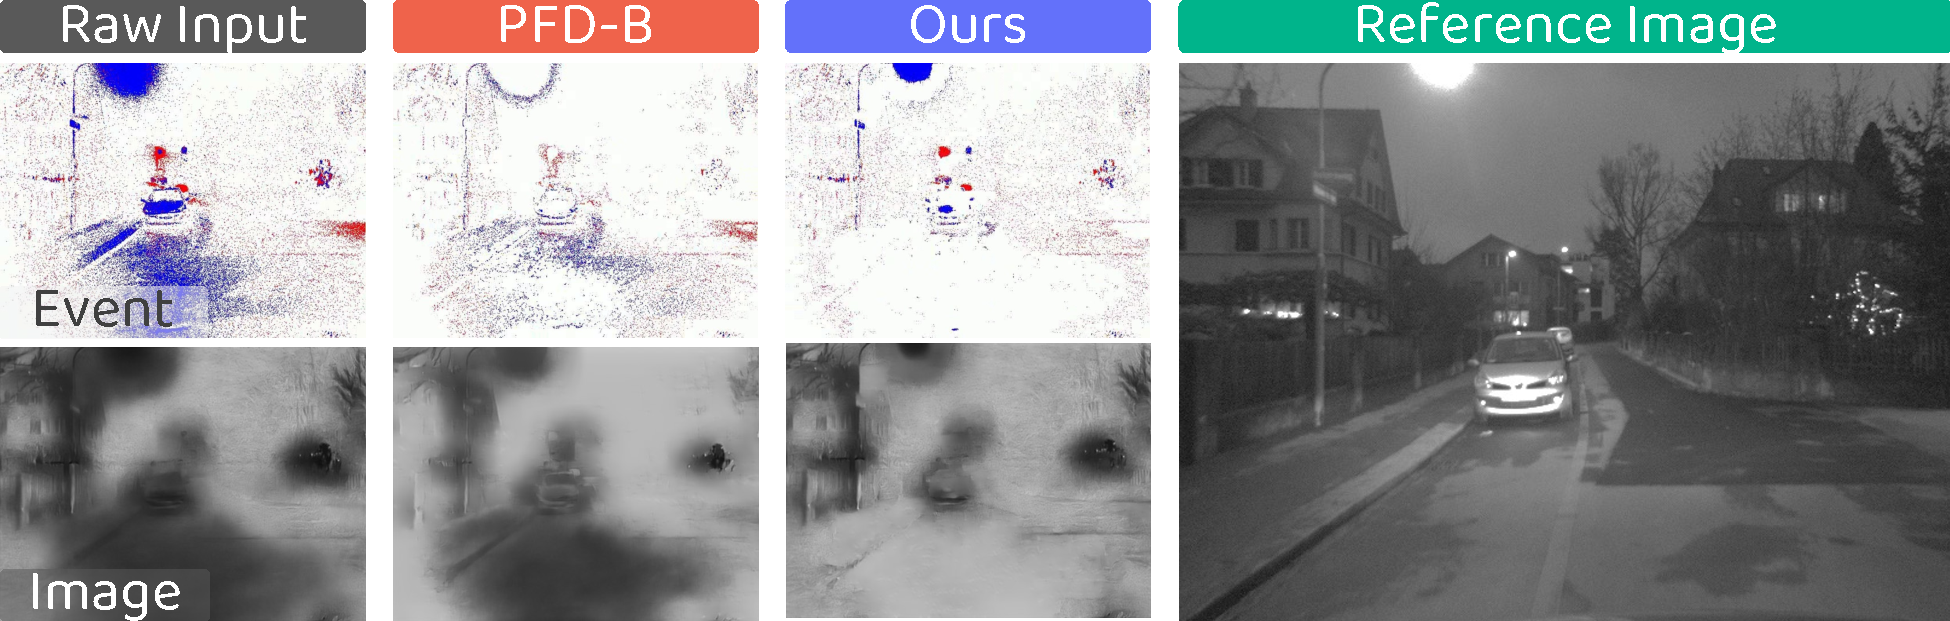
\includegraphics[width=\columnwidth]{figures/image_reconstruction.pdf}
    \vspace{-0.65cm}
    \caption{\textbf{Downstream task comparisons} for event-based imaging. We use SPADE-E2VID~\cite{cadena2021spade} to reconstruct images from both raw and our de-flared event streams on a challenging DSEC scene.}
    \label{fig:image_reconstruction}
    \vspace{-0.1cm}
\end{figure}
Collectively, these ablations confirm that the success of \textbf{E-Deflare} arises from principled physical modeling: (1) maintaining correct light source semantics in training targets, and (2) implementing the non-linear event suppression mechanism derived from the irradiance-domain interaction model.


\begin{table*}[t]
    \centering
    \caption{\textbf{Ablation study on the E-Flare-R dataset}. We evaluate three variants to analyze our core design choices. The final row shows the improvement of our full model over the best ablated variant ($\downarrow$: lower is better, $\uparrow$: higher is better). Ch. = Chamfer Distance; Gau. = Gaussian Distance; PM2/PM4 = Pooled MSE at scales 2/4.}
    \vspace{-0.3cm}
    \label{tab:ablation_main}
    \small
    \resizebox{\textwidth}{!}{%
    \begin{tabular}{lcccccccc}
    \toprule
    \textbf{Config.} & ~~Ch.$\downarrow$~~ & ~~Gau.$\downarrow$~~ & ~MSE$\downarrow$~ & ~PM2$\downarrow$~ & ~PM4$\downarrow$~ & ~R-F1$\uparrow$~ & ~T-F1$\uparrow$~ & ~TP-F1$\uparrow$~
    \\
    \midrule
    \textcolor{gray}{$\bullet$}~\textcolor{gray}{Raw Input} & \cellcolor{gray!20}\textcolor{gray}{$1.7855$} & \cellcolor{gray!20}\textcolor{gray}{$0.7170$} & \cellcolor{gray!20}\textcolor{gray}{$0.8158$} & \cellcolor{gray!20}\textcolor{gray}{$0.3431$} & \cellcolor{gray!20}\textcolor{gray}{$0.3266$} & \cellcolor{gray!20}\textcolor{gray}{$0.2299$} & \cellcolor{gray!20}\textcolor{gray}{$0.2915$} & \cellcolor{gray!20}\textcolor{gray}{$0.3093$}
    \\\midrule
    \textcolor{ev_green}{$\bullet$}~No Light & $1.9745$ & $0.8487$ & $0.1951$ & $0.0843$ & $0.0806$ & $0.0189$ & $0.0459$ & $0.0709$
    \\
    \textcolor{ev_red}{$\bullet$}~Simple & \cellcolor{ev_red!20}$1.3434$ & \cellcolor{ev_red!20}$0.5564$ & \cellcolor{ev_red!20}$0.1816$ & \cellcolor{ev_red!20}$0.0734$ & \cellcolor{ev_red!20}$0.0688$ & \cellcolor{ev_red!20}$0.2703$ & \cellcolor{ev_red!20}$0.2768$ & \cellcolor{ev_red!20}$0.2644$
    \\
    % \textcolor{ev_red}{$\bullet$}~Full Model $+$ Jitter & $1.6811$ & $0.7203$ & $0.2020$ & $0.0834$ & $0.0788$ & $0.1567$ & $0.2001$ & $0.2103$
    % \\
    \midrule
    \textcolor{ev_blue}{$\bullet$}~\textbf{Full Model (Ours)} & \cellcolor{ev_blue!20}$\mathbf{1.1368}$ & \cellcolor{ev_blue!20}$\mathbf{0.4651}$ & \cellcolor{ev_blue!20}$\mathbf{0.1741}$ & \cellcolor{ev_blue!20}$\mathbf{0.0690}$ & \cellcolor{ev_blue!20}$\mathbf{0.0644}$ & \cellcolor{ev_blue!20}$\mathbf{0.3498}$ & \cellcolor{ev_blue!20}$\mathbf{0.3386}$ & \cellcolor{ev_blue!20}$\mathbf{0.3011}$
    \\
    \emph{Improvement (\%)} $\uparrow$ & $15.4\%$$\uparrow$ & $16.4\%$$\uparrow$ & $4.1\%$$\uparrow$ & $6.0\%$$\uparrow$ & $6.4\%$$\uparrow$ & $29.4\%$$\uparrow$ & $22.3\%$$\uparrow$ & $13.9\%$$\uparrow$
    \\
    \bottomrule
    \end{tabular}%
    }%
\vspace{-0.2cm}
\end{table*}



\subsection{Downstream Task Evaluations}
\label{sec:downstream}

To validate the generalizability of our framework, we evaluate \textbf{E-Deflare} on two high-level tasks: image reconstruction and 3D scene reconstruction.


\begin{table}[t]
    \centering
    \caption{\textbf{Downstream task comparisons} for event-based 3D reconstruction. We use Event3DGS~\cite{han2024event} to reconstruct scenes and evaluate the quality of novel view synthesis. $\uparrow$: higher is better.}
    \label{tab:3dgs_quant}
    \small
    \resizebox{\columnwidth}{!}{%
    \begin{tabular}{r|c|ccc|c}
    \toprule
    \textbf{Metric} & \textcolor{gray}{Original} & EFR & PFD-A & PFD-B & \textbf{Ours}
    \\
    \midrule
    PSNR $\uparrow$ & \cellcolor{gray!20}\textcolor{gray}{$13.72$} & \cellcolor{ev_red!20}$13.74$ & $13.11$ & $13.32$ & \cellcolor{ev_blue!20}$\mathbf{13.78}$
    \\
    SSIM $\uparrow$ & \cellcolor{gray!20}\textcolor{gray}{$0.765$} & $0.741$ & \cellcolor{ev_red!20}$0.743$ & $0.734$ & \cellcolor{ev_blue!20}$\mathbf{0.792}$
    \\
    \bottomrule
    \end{tabular}}
    \vspace{-0.1cm}
\end{table}
\noindent\textbf{Event-based Imaging.}
We first assess the impact of de-flaring on event-to-image reconstruction using the state-of-the-art SPADE-E2VID framework~\cite{cadena2021spade}. Fig.~\ref{fig:image_reconstruction} shows results on challenging sequences in \textbf{DSEC-Flare}. Images reconstructed from raw, flare-corrupted events exhibit strong flare patterns, obscuring fine scene details. In contrast, images reconstructed from our de-flared events recover cleaner and accurate illumination, revealing significant visual improvement. These results demonstrate that \textbf{E-Deflare} serves as an effective pre-processing step, substantially enhancing the clarity and usability of event data for imaging applications.




% \noindent\textbf{Event-based 3D Reconstruction.}
% To demonstrate the practical impact of our method, we conduct a rigorous quantitative evaluation on the downstream task of event-based 3D reconstruction. As no standard benchmark with flare artifacts exists for this task, we created one by synthesizing paired event datasets using the popular LEGO scene from the NeRF-synthetic \cite{mildenhall2021nerf} dataset, following the simulation methodology of PECS \cite{han2024physical}.

% Using the method from Event3DGS~\cite{han2024event}, we reconstruct a 3D scene from the original flare-corrupted input, our de-flared output, and the outputs from baseline methods. We then evaluate the quality of each reconstruction by rendering novel views and comparing them against the pristine ground truth. To ensure fairness, the background is color-normalized during metric calculation.

% The results in Table~\ref{tab:3dgs_quant} reveal that naive de-flaring can be detrimental. Most baselines fail to improve reconstruction, with some even degrading performance below the original input. In stark contrast, our method is the only one to provide a clear and consistent improvement, boosting the SSIM from $0.765$ to a state-of-the-art $\mathbf{0.792}$ where all others falter. This powerfully demonstrates that our approach provides a cleaner, more reliable input that directly benefits downstream 3D perception.

\noindent\textbf{Event-based 3D Reconstruction.}
To demonstrate the practical impact of our method, we conduct a rigorous quantitative evaluation on event-based 3D reconstruction. As no standard benchmark with flare artifacts exists for this task, we synthesized a paired event dataset from the popular LEGO scene of NeRF-synthetic~\cite{mildenhall2021nerf}, following the simulation methodology of PECS~\cite{han2024physical}. The experimental process involves reconstructing a 3D scene from various event streams (the original flare-corrupted input, our de-flared output, and outputs from baseline methods) using Event3DGS~\cite{han2024event}. We then evaluate the reconstruction by rendering novel views and comparing them against the pristine ground truth, with background color normalization for a fair comparison.



\begin{figure}[t]
    \centering
    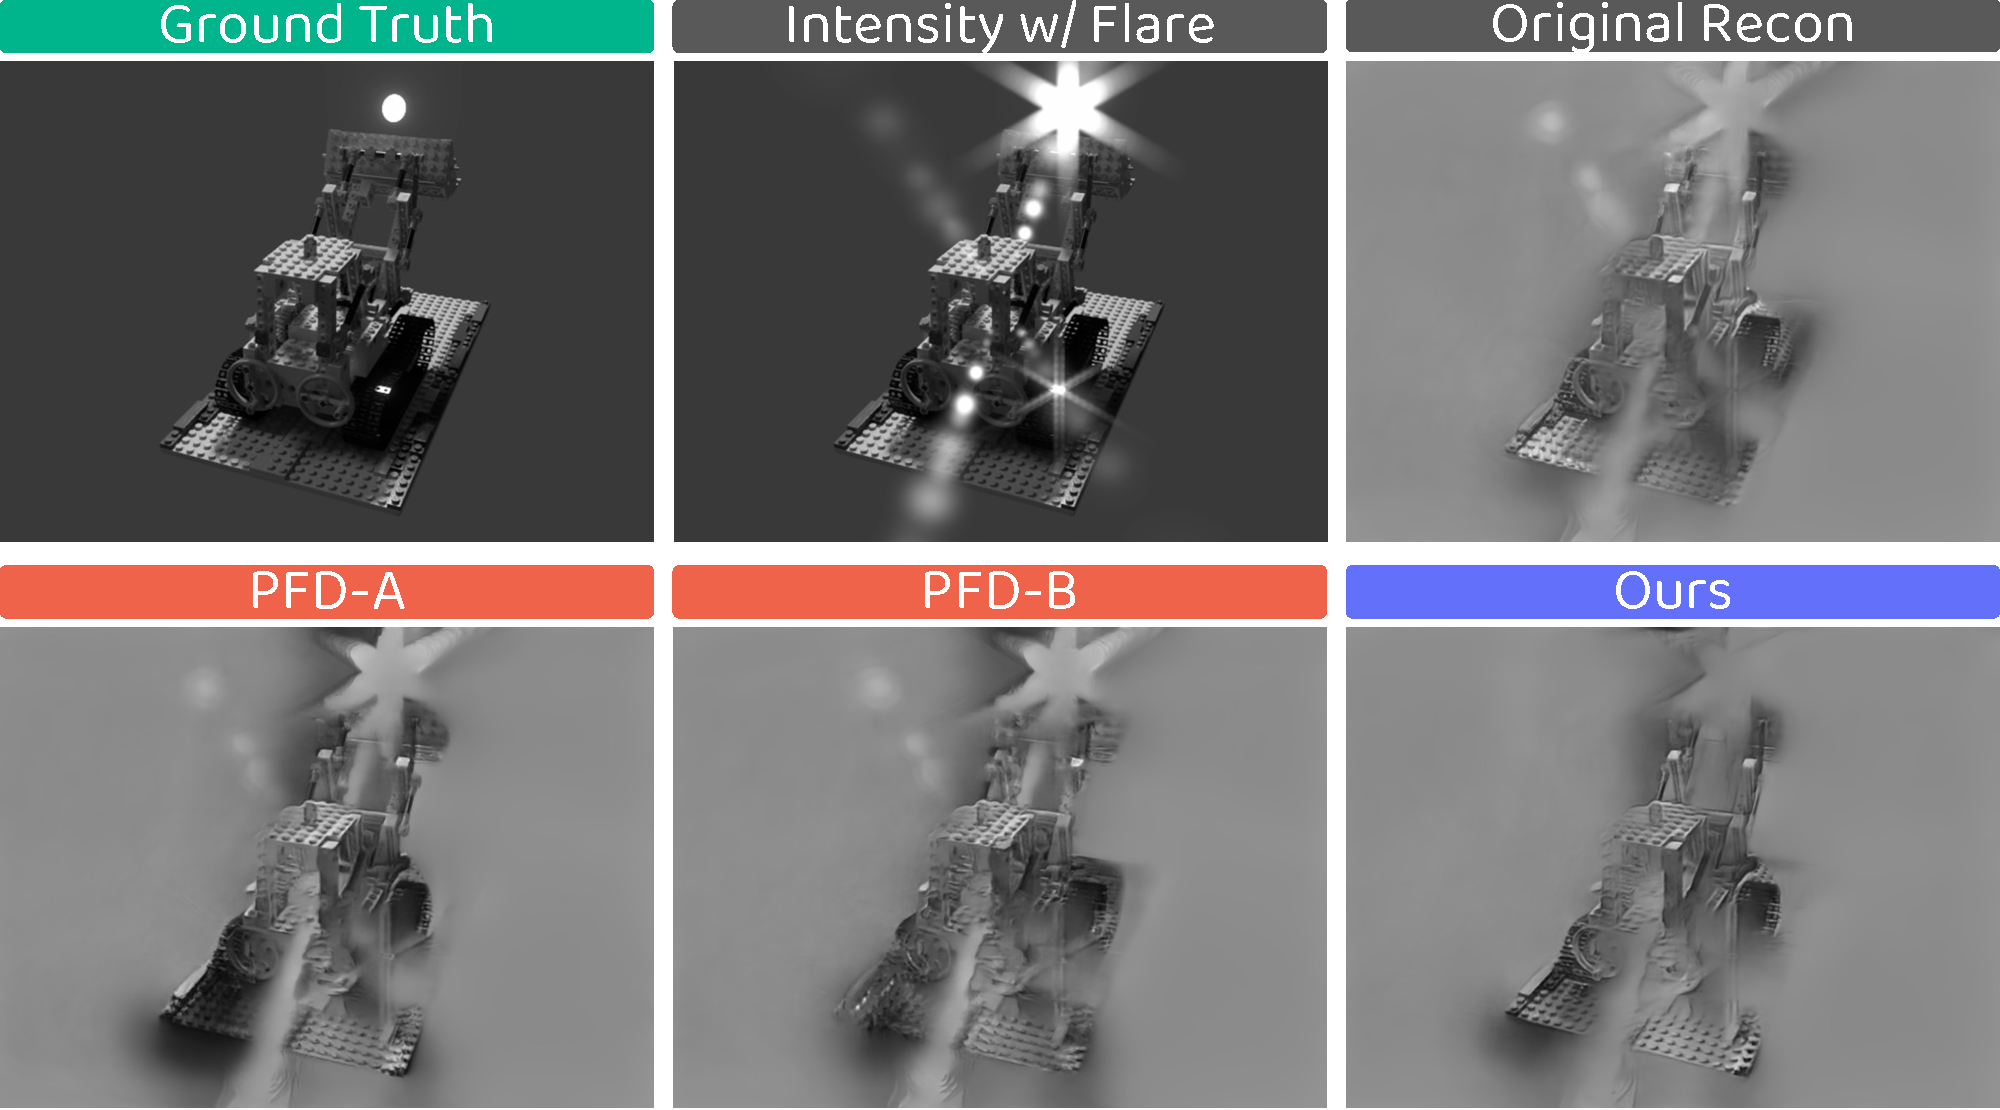
\includegraphics[width=\columnwidth]{figures/3D_reconstruction.pdf}
    \vspace{-0.65cm}
    \caption{\textbf{Downstream task comparisons} for event-based 3D reconstruction. We visualize the rendered views from 3D scenes reconstructed using the outputs of different de-flaring methods.}
    \label{fig:3dgs_qual}
    \vspace{-0.1cm}
\end{figure}
The results in Table~\ref{tab:3dgs_quant} reveal that naive de-flaring can be detrimental. Most baselines fail to improve reconstruction, with some even degrading performance below the original input. In contrast, our method is the only one providing a clear and consistent improvement, boosting the SSIM from $0.765$ to a state-of-the-art $\mathbf{0.792}$. This powerfully demonstrates that our approach provides a cleaner, more reliable input that directly and substantially benefits downstream 3D perception tasks.


%old version, the bg have different color

% % --- Table for 3D Reconstruction ---
% \begin{table}[t]
%     \centering
%     \caption{Quantitative results for the downstream task of event-based 3D reconstruction. Our method leads to higher quality novel view synthesis, evaluated by PSNR, SSIM, and LPIPS metrics.}
%     \label{tab:3dgs_quant}
%     \small
%     % The 'booktabs' package is needed for \toprule, \midrule, \bottomrule
%     \begin{tabular*}{\columnwidth}{l@{\extracolsep{\fill}}ccccc}
%     \toprule
%     Metric & Original & EFR & PFD-A & PFD-B & \textbf{Ours} \\
%     \midrule
%     PSNR $\uparrow$ & 14.29 & 14.22 & 13.67 & 13.92 & \textbf{14.32} \\
%     SSIM $\uparrow$      & 0.759 & 0.747 & 0.735 & 0.739 & \textbf{0.777} \\
%     LPIPS $\downarrow$   & \textbf{0.273} & 0.308 & 0.287 & 0.298 & 0.285 \\
%     \bottomrule
%     \end{tabular*}
% \end{table}

\section{Conclusion}
\label{sec:conclusion}

We introduced \textbf{E-Deflare}, the first systematic framework for lens flare in event camera data. At its core, a physics-based forward model explains how flare non-linearly suppresses background events and guides both the \textbf{E-Flare2.7K} simulation dataset and \textbf{E-Flare-R}, the first paired real-world test set. Together with \textbf{DSEC-Flare}, they form the \textbf{E-Deflare Benchmark}. Experiments with a standard 3D U-Net validate the theory and data across synthetic and real settings, achieving state-of-the-art de-flaring while preserving valid events under challenging real-world flare conditions and improving downstream event camera imaging. Future work will study stronger network architectures and larger paired real-world datasets.


{
    \small
    \bibliographystyle{ieeenat_fullname}
    \bibliography{main}
}

\end{document}
